\documentclass[11pt,spanish] {article}
\def\spanishoptions{mexico}
\usepackage{mathptmx}
\usepackage{mwe,tikz}
\usepackage[percent]{overpic}
\usepackage[margin=0.5in]{geometry}
%~ \usepackage[spanish,es-noshorthands,es-ucroman]{babel}
\usepackage[spanish]{babel}
\usepackage{csvsimple}
\selectlanguage{spanish}
\usepackage[utf8]{inputenc}
%~ \usepackage{fancyhdr}
\usepackage[cm]{fullpage}
\usepackage{tabu}
\usepackage{hyperref}
%~ \pagestyle{fancy}
\usepackage[section]{placeins}
\usepackage{titlesec}
\usepackage{multirow}
\usepackage{graphicx}
\usepackage{makecell}
\usepackage{floatrow}
\usepackage{caption}
\usepackage{xcolor,colortbl}
%~ \usepackage{titling}
%~ \setlength{\droptitle}{-3cm}
\makeatletter
\def\input@path{{./public/latex/}}
%or: \def\input@path{{/path/to/folder/}{/path/to/other/folder/}}
\makeatother
\DeclareRobustCommand{\fecha}{02/ene/2021
}
\DeclareRobustCommand{\fechaformat}{25/ene/2021
}
\DeclareRobustCommand{\fechapasada}{18/ene/2021
}
\DeclareRobustCommand{\pronodiariocomentario}{
}
\DeclareRobustCommand{\comentariofinal}{
}
\DeclareRobustCommand{\fechaproximo}{lunes 01/mar/2021
}
\DeclareRobustCommand{\synoptext}{Se destaca pocos eventos de importancia y sobre áreas de respuesta
retardada. Las lluvias registradas en la última semana no alcanzan
magnitud como para alterar las tendencias hidrométricas en la región.
}
\DeclareRobustCommand{\pronodiario}{\begin{tabular}{|c|c|c|c|c|}
\hline
\textbf{Fecha} & \textbf{B. Negra} & \textbf{Concepción} & \textbf{P. Pilcomayo} & \textbf{Formosa} \\
\hline
\textbf{HOY} &  2,46 &  2,32 &  3,86 &  5,23 \\
\hline
\textbf{27/02} &  2,46 &  2,29 &  3,8 &  5,08 \\
\hline
\textbf{28/02} &  2,47 &  2,27 &  3,7 &  4,98 \\
\hline
\textbf{01/03} &  2,47 &  2,26 &  3,6 &  4,88 \\
\hline
\textbf{02/03} &  2,48 &  2,25 &  3,51 &  4,78 \\
\hline
\textbf{03/03} &  2,49 &  2,24 &  3,41 &  4,7 \\
\hline
\textbf{04/03} &  2,5 &  2,23 &  3,32 &  4,62 \\
\hline
\textbf{05/03} &  2,51 &  2,23 &  3,22 &  4,55 \\
\hline
\textbf{06/03} &  2,52 &  2,24 &  3,17 &  4,48 \\
\hline
\end{tabular}}
\DeclareRobustCommand{\pronomensual}{\begin{tabular}{|c|c|c|c|c|}
\hline
\textbf{Mes} & \textbf{B. Negra} & \textbf{Concepción} & \textbf{P. Pilcomayo} & \textbf{Formosa} \\
\hline
\textbf{febrero} & 2,42 & 3,02 & 4,56 & 5,41 \\
\hline
\textbf{marzo} & 2,62 & 2,44 & 3,1 & 4,21 \\
\hline
\textbf{abril} & 2,87 & 2,96 & 3,33 & 4,08 \\
\hline
\textbf{mayo} & 3,15 & 3,15 & 3,71 & 4,36 \\
\hline
\end{tabular}}
\DeclareRobustCommand{\horizonte}{31/may/2021
}
\providecommand{\tightlist}{%
  \setlength{\itemsep}{0pt}\setlength{\parskip}{0pt}}
%~ \headheight 0pt
\setlength{\footskip}{10pt}
%~ \headsep 1pt 
\titlespacing*{\section}{0pt}{0ex}{0ex}
\graphicspath{{/home/alerta5/44-NODEJS_APIS/informe_complementario/public/latex/}}
\usepackage{tabularx}
\begin{document}
\captionsetup{labelformat=empty}
%~ \paragraph*{}
%~ \begin{center}
%~ \begin{tabularx}{\textwidth}{|c|>{\centering\arraybackslash}X|c|}
	%~ \hline
	%~ \multirow{3}{*}{
\includegraphics[width=5cm]{Logo_MOSP_2020.png}} & \textbf{\large{Instituto Nacional del Agua}} & \multirow{3}{*}{
\includegraphics[width=2.6cm,height=1.5cm]{logo_ina_crop.png}}  \\
	%~ & \textbf{\large{Subgerencia de Sistemas de Información y}} & \\ 
	%~ & \textbf{\large{Alerta Hidrológico}} & \\
	%~ \hline
	   %~ \makecell{\Large{\textbf{Informe de Situación}}} &  \makecell{\Large{\textbf{Cuenca del río Paraguay}}} & \fecha \\
	%~ \hline
%~ \end{tabularx}

%~ Ing. Juan Borús, Lic. Maximiliano Vita Sánchez,Dr. Leandro Giordano, Lic. Juan Bianchi
%~ \end{center}
\begingroup
\begin{center}
\renewcommand{\arraystretch}{0.8}
\begin{tabularx}{\textwidth}{|c|>{\centering\arraybackslash}X|c|}
	\hline
	\multirow{5}{*}{
\includegraphics[height=1.7cm]{escudo_argentina.png}} & \textbf{\small{Ministerio de Obras Públicas}} & \multirow{5}{*}{
\includegraphics[width=2.6cm,height=1.3cm]{logo_ina_crop.png}}  \\
	& \textbf{\small{Secretaría de Infraestructura y Política Hídrica}} & \\
	& \textbf{\small{Subsecretaría de Obras Hidráulicas}} & \\
	& \textbf{\small{Instituto Nacional del Agua}} & \\ 
	& \textbf{\scriptsize{2021 - Año de Homenaje al Premio Nobel de Medicina Dr. César Milstein}} & \\ 
	\hline
	   \makecell{\textbf{Informe de Situación}} &  \makecell{\Large{\textbf{Cuenca del río Paraguay}}} &  \fecha \\
	\hline
\end{tabularx}
Ing. Juan Borús, Lic. Maximiliano Vita Sánchez, Dr. Leandro Giordano, Mg. Juan Bianchi
\end{center}
\endgroup
%~ \paragraph*{}
%~ \vspace{1cm}
\subsection{Acumulados semanales de lluvia}
\begin{tabular}{|c|c|}
	\hline
	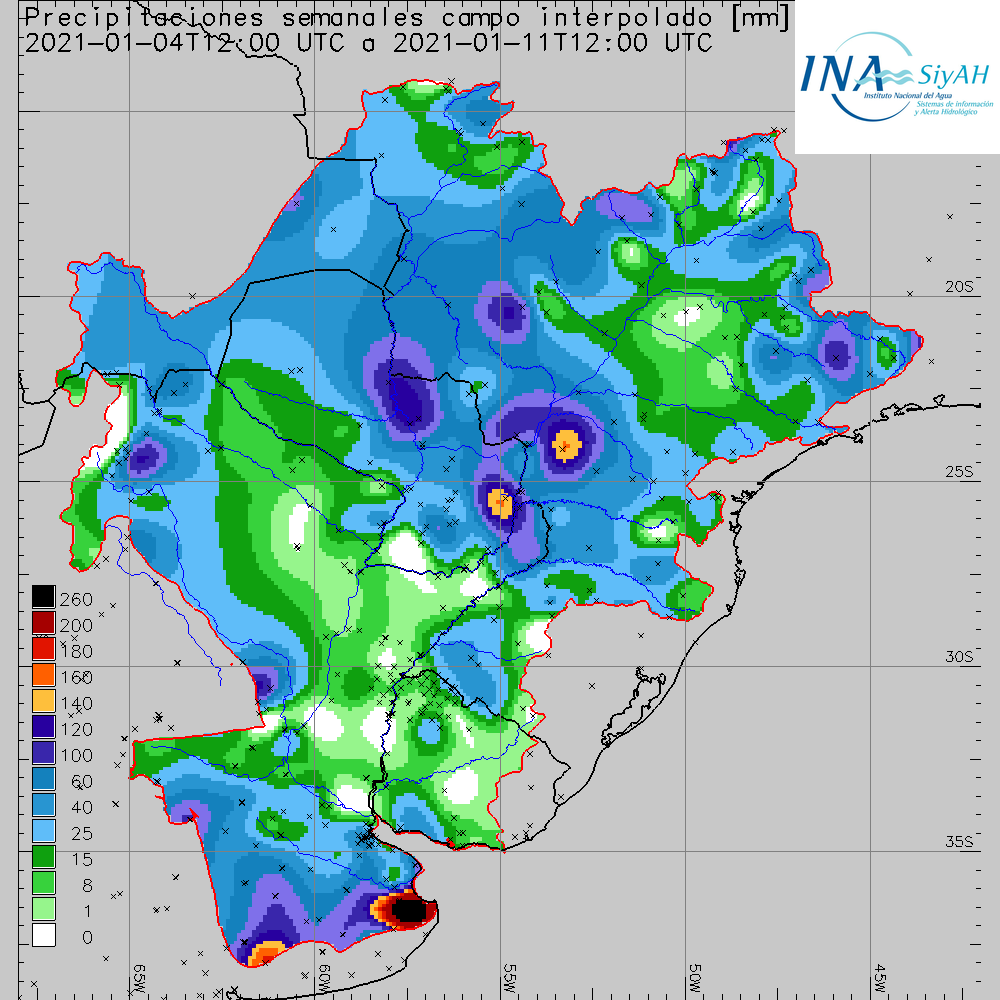
\includegraphics[width=8.5cm]{synop_pasada.png} & 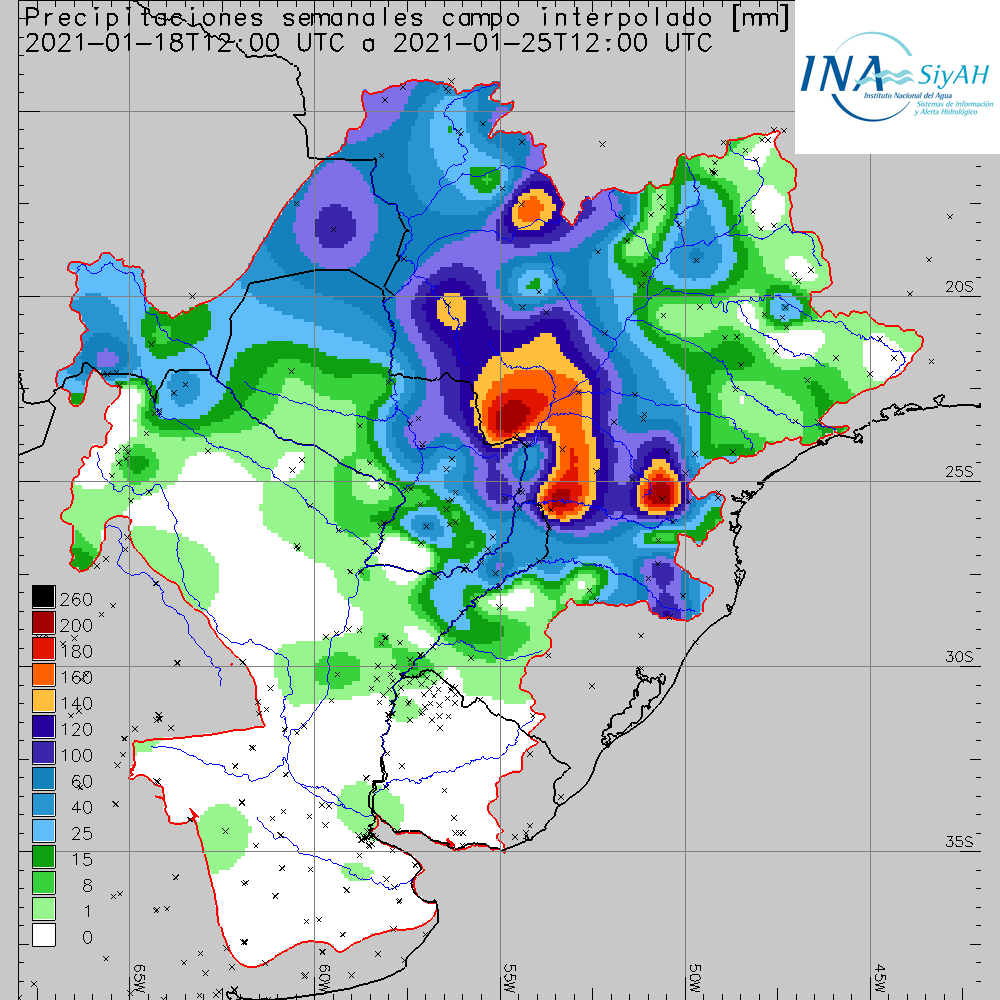
\includegraphics[width=8.5cm]{synop_presente.png} \\
	\hline
	Lluvias semanales acumuladas al \fechapasada & Lluvias acumuladas semanales al \fechaformat \\
	\hline
\end{tabular}

Los niveles esperados son (en metros):

\begin{center}

\pronodiario

\emph{En sombreado niveles por encima de los respectivos de alerta (amarillo) o evacuación (rojo)}
\end{center}

\pronodiariocomentario

Para el recinto de defensa de la ciudad de Formosa se actualiza la condición de las estaciones
de bombeo en función del nivel fluvial, actualizando la siguiente tabla:
\begin{center}
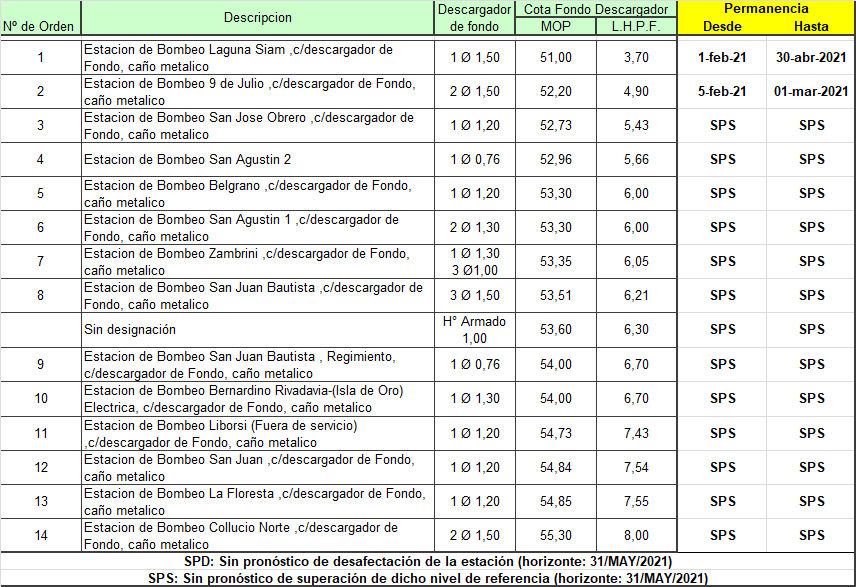
\includegraphics[width=13.5cm]{tabla_bombas.png}
\end{center}
Los niveles medios mensuales esperados son (en metros, horizonte \horizonte):
\begin{center}
\pronomensual
\end{center}
\comentariofinal

El monitoreo permanente continuará en los próximos días y se informará sobre los cambios en la
expectativa y pronósticos hidrométricos. La actualización es diaria. El mensaje completo será
preparado el próximo \emph{\fechaproximo} y presentado en la página web.

\pagebreak
\begin{center}
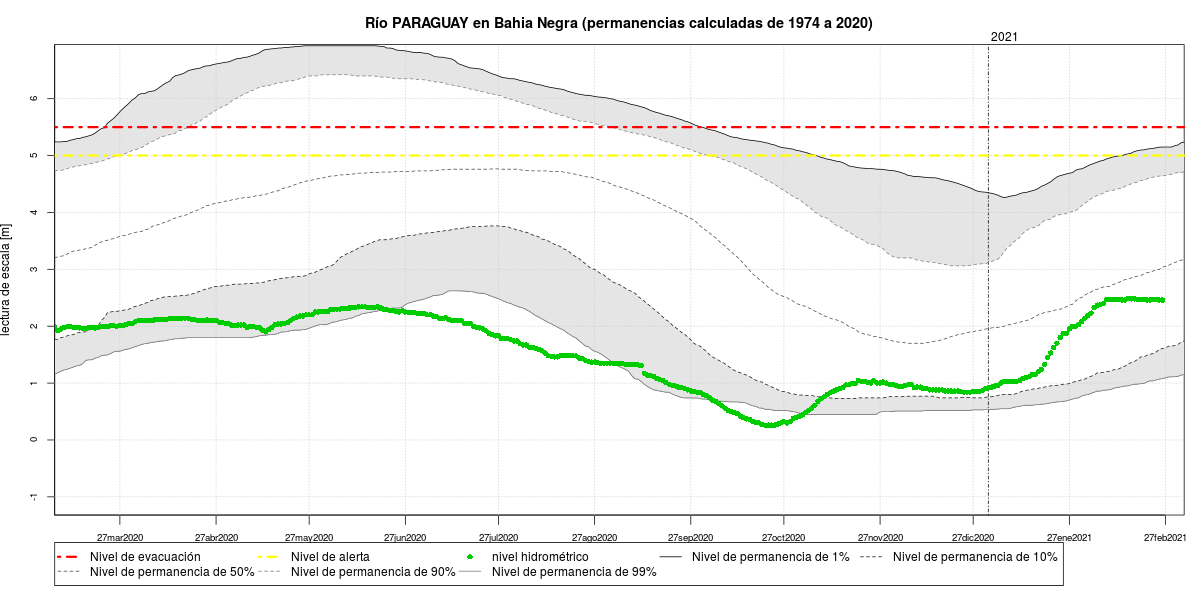
\includegraphics[width=17cm]{niveles_bneg.png}

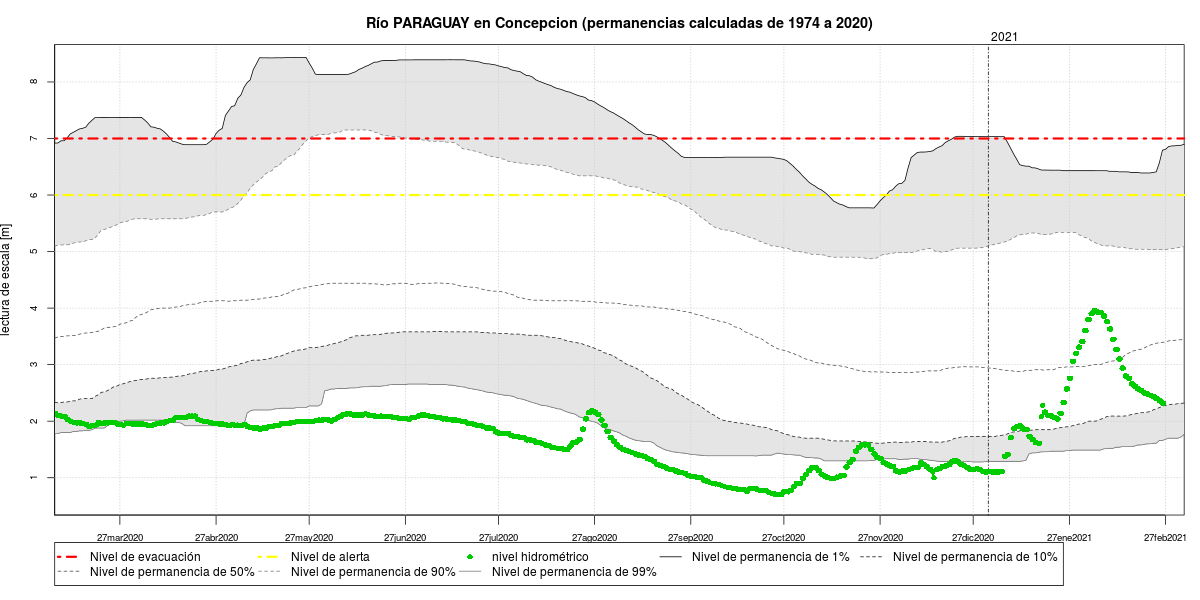
\includegraphics[width=17cm]{niveles_conc.png}

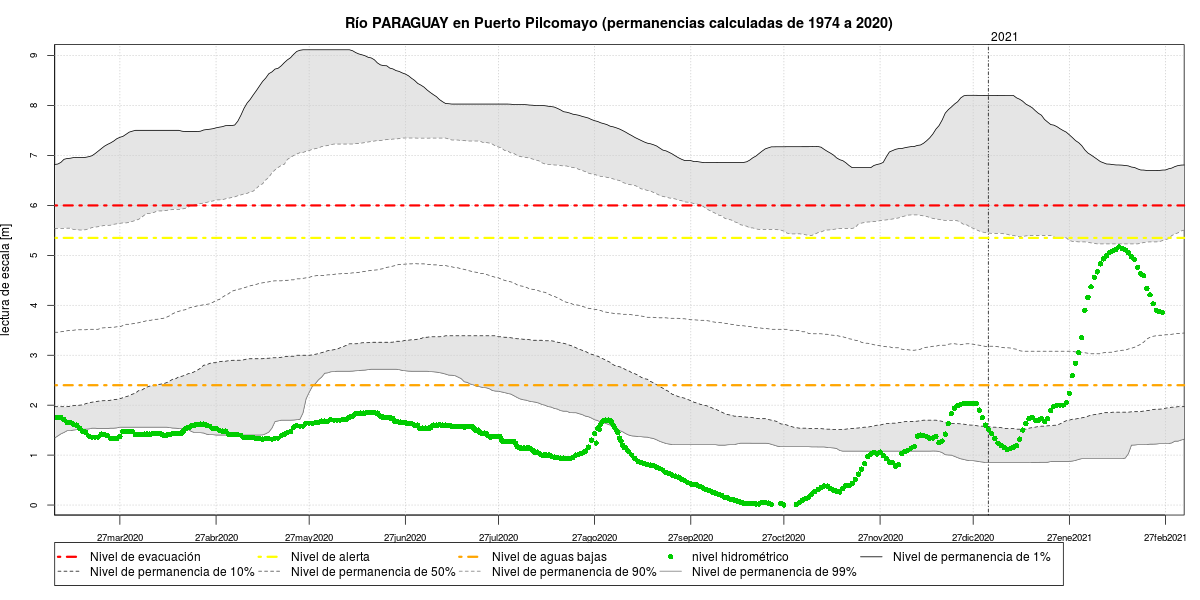
\includegraphics[width=17cm]{niveles_pilc.png}

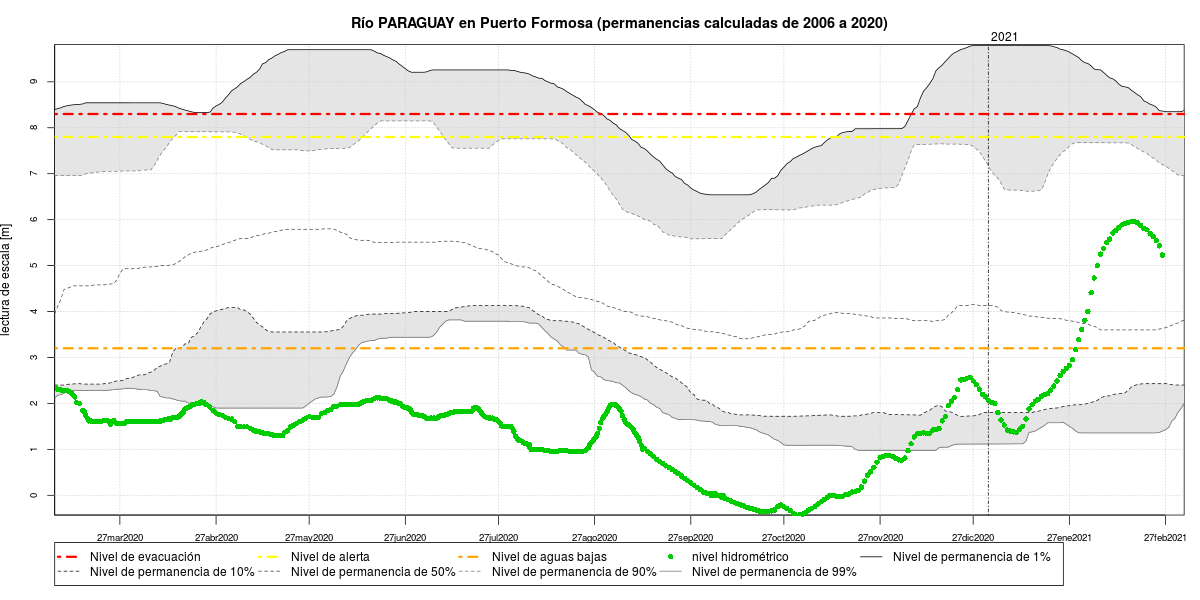
\includegraphics[width=17cm]{niveles_form.png}
\end{center}
\end{document}

